\documentclass{article}

\usepackage{graphics}
\usepackage[vcentering]{geometry}

\geometry{papersize={5.4in,3.2in}, top=0in, bottom=0in, left=0in, right=0in}

\pagestyle{empty}

\usepackage{tikz}
\usetikzlibrary{
	arrows,shapes,decorations.pathmorphing,backgrounds,positioning,fit,calc,scopes
}


\tikzset{
	auto,
	compartment/.style={
		rectangle, minimum size=9mm, rounded corners=2mm,
		thick, draw=black!15, top color=white,bottom color=black!30
	},
	%
	bigcompartment/.style={
		rectangle, minimum size=20mm, rounded corners=2mm,
		thick, draw=black!30, top color=white,bottom color=black!20
	},
	%
	point/.style={
		circle, inner sep=2pt, fill=black!5
	},
	%
	mytextbox/.style={
		rectangle, text=black!50, thin, 
		draw=white, top color=white,bottom color=white, fill=white
	}
}


\begin{document}

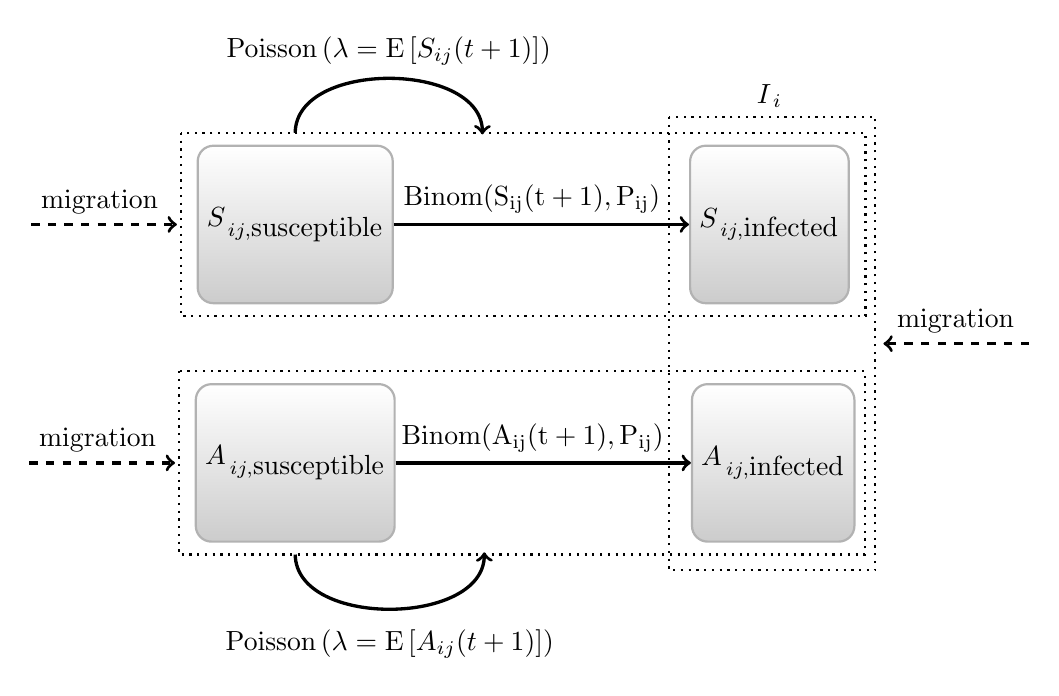
\begin{tikzpicture}
    \node(S)[bigcompartment]{$S_{\,ij,\textrm{susceptible}}$};
    \node(StoSI)[right=of S]{};
    \node(SI)[bigcompartment, right=2.5cm of StoSI]{$S_{\,ij,\textrm{infected}}$};
    \draw[->, very thick] (S) -- node [text width=3.5cm, midway, above] {$\mathrm{\mathrm{Binom}(S_{ij}(t+1), P_{ij})}$} (SI); 
    \node(A)[bigcompartment, below=of S]{$A_{\,ij,\textrm{susceptible}}$};
    \node(AtoAI)[right=of A]{};
    \node(AI)[bigcompartment, right=2.5cm of AtoAI]{$A_{\,ij,\textrm{infected}}$};
    \draw[->, very thick] (A) -- node [text width=3.6cm, midway, above] {$\mathrm{\mathrm{Binom}(A_{ij}(t+1), P_{ij})}$} (AI); 
    \node(Sextra)[left=of S]{};
    \draw[->, very thick, dashed] ([xshift=-1.1cm]Sextra.east)  -- node [text width=1.6cm, midway, above] {migration}  ([xshift=-0.25cm]S.west);
    \node(Aextra)[left=of A]{};
    \draw[->, very thick, dashed] ([xshift=-1.1cm]Aextra.east)  -- node [text width=1.6cm, midway, above] {migration}     ([xshift=-0.25cm]A.west);
    \draw[thick,dotted] ($(SI.north west)+(-0.25,0.35)$) rectangle ($(AI.south east)+(0.25,-0.35)$);
    \draw[thick,dotted] ($(S.north west)+(-0.2,0.15)$) rectangle ($(SI.south east)+(0.2,-0.15)$);
    \draw[thick,dotted] ($(A.north west)+(-0.2,0.15)$) rectangle ($(AI.south east)+(0.12,-0.15)$);
    \node(I) at ($(AI)!0.5!(SI)$){};
    \node[above] at ([yshift=0.35cm] SI.north){$I_{\,i}$};
    \node(Iextra)[right=of I]{};
    \draw[->, very thick, dashed] ([xshift=1.9cm]Iextra.east) -- node [text width=1.5cm, midway, above] {migration}  ([xshift=1.3cm]I.east);
    \draw[->, very thick] ([yshift=0.15cm]S.north) to [bend left=90]([yshift=1.02cm]StoSI.north);
    \draw[->, very thick] ([yshift=-0.15cm]A.south) to [bend right=90]([yshift=-1.26cm]AtoAI.north);
    \node(Sbirth) at ([yshift=2.2cm]$(S)!0.5!(StoSI)$){$\mathrm{Poisson}\left(\lambda=\mathrm{E}\left[S_{ij}(t+1)\right]\right)$};
    \node(Abirth) at ([yshift=-2.3cm]$(A)!0.5!(AtoAI)$){$\mathrm{Poisson}\left(\lambda=\mathrm{E}\left[A_{ij}(t+1)\right]\right)$};
\end{tikzpicture}

\end{document}
